% Options for packages loaded elsewhere
\PassOptionsToPackage{unicode}{hyperref}
\PassOptionsToPackage{hyphens}{url}
\documentclass[
  11pt,
]{article}
\usepackage{xcolor}
\usepackage[margin=1in]{geometry}
\usepackage{amsmath,amssymb}
\setcounter{secnumdepth}{-\maxdimen} % remove section numbering
\usepackage{iftex}
\ifPDFTeX
  \usepackage[T1]{fontenc}
  \usepackage[utf8]{inputenc}
  \usepackage{textcomp} % provide euro and other symbols
\else % if luatex or xetex
  \usepackage{unicode-math} % this also loads fontspec
  \defaultfontfeatures{Scale=MatchLowercase}
  \defaultfontfeatures[\rmfamily]{Ligatures=TeX,Scale=1}
\fi
\usepackage{lmodern}
\ifPDFTeX\else
  % xetex/luatex font selection
\fi
% Use upquote if available, for straight quotes in verbatim environments
\IfFileExists{upquote.sty}{\usepackage{upquote}}{}
\IfFileExists{microtype.sty}{% use microtype if available
  \usepackage[]{microtype}
  \UseMicrotypeSet[protrusion]{basicmath} % disable protrusion for tt fonts
}{}
\makeatletter
\@ifundefined{KOMAClassName}{% if non-KOMA class
  \IfFileExists{parskip.sty}{%
    \usepackage{parskip}
  }{% else
    \setlength{\parindent}{0pt}
    \setlength{\parskip}{6pt plus 2pt minus 1pt}}
}{% if KOMA class
  \KOMAoptions{parskip=half}}
\makeatother
\usepackage{color}
\usepackage{fancyvrb}
\newcommand{\VerbBar}{|}
\newcommand{\VERB}{\Verb[commandchars=\\\{\}]}
\DefineVerbatimEnvironment{Highlighting}{Verbatim}{commandchars=\\\{\}}
% Add ',fontsize=\small' for more characters per line
\usepackage{framed}
\definecolor{shadecolor}{RGB}{248,248,248}
\newenvironment{Shaded}{\begin{snugshade}}{\end{snugshade}}
\newcommand{\AlertTok}[1]{\textcolor[rgb]{0.94,0.16,0.16}{#1}}
\newcommand{\AnnotationTok}[1]{\textcolor[rgb]{0.56,0.35,0.01}{\textbf{\textit{#1}}}}
\newcommand{\AttributeTok}[1]{\textcolor[rgb]{0.13,0.29,0.53}{#1}}
\newcommand{\BaseNTok}[1]{\textcolor[rgb]{0.00,0.00,0.81}{#1}}
\newcommand{\BuiltInTok}[1]{#1}
\newcommand{\CharTok}[1]{\textcolor[rgb]{0.31,0.60,0.02}{#1}}
\newcommand{\CommentTok}[1]{\textcolor[rgb]{0.56,0.35,0.01}{\textit{#1}}}
\newcommand{\CommentVarTok}[1]{\textcolor[rgb]{0.56,0.35,0.01}{\textbf{\textit{#1}}}}
\newcommand{\ConstantTok}[1]{\textcolor[rgb]{0.56,0.35,0.01}{#1}}
\newcommand{\ControlFlowTok}[1]{\textcolor[rgb]{0.13,0.29,0.53}{\textbf{#1}}}
\newcommand{\DataTypeTok}[1]{\textcolor[rgb]{0.13,0.29,0.53}{#1}}
\newcommand{\DecValTok}[1]{\textcolor[rgb]{0.00,0.00,0.81}{#1}}
\newcommand{\DocumentationTok}[1]{\textcolor[rgb]{0.56,0.35,0.01}{\textbf{\textit{#1}}}}
\newcommand{\ErrorTok}[1]{\textcolor[rgb]{0.64,0.00,0.00}{\textbf{#1}}}
\newcommand{\ExtensionTok}[1]{#1}
\newcommand{\FloatTok}[1]{\textcolor[rgb]{0.00,0.00,0.81}{#1}}
\newcommand{\FunctionTok}[1]{\textcolor[rgb]{0.13,0.29,0.53}{\textbf{#1}}}
\newcommand{\ImportTok}[1]{#1}
\newcommand{\InformationTok}[1]{\textcolor[rgb]{0.56,0.35,0.01}{\textbf{\textit{#1}}}}
\newcommand{\KeywordTok}[1]{\textcolor[rgb]{0.13,0.29,0.53}{\textbf{#1}}}
\newcommand{\NormalTok}[1]{#1}
\newcommand{\OperatorTok}[1]{\textcolor[rgb]{0.81,0.36,0.00}{\textbf{#1}}}
\newcommand{\OtherTok}[1]{\textcolor[rgb]{0.56,0.35,0.01}{#1}}
\newcommand{\PreprocessorTok}[1]{\textcolor[rgb]{0.56,0.35,0.01}{\textit{#1}}}
\newcommand{\RegionMarkerTok}[1]{#1}
\newcommand{\SpecialCharTok}[1]{\textcolor[rgb]{0.81,0.36,0.00}{\textbf{#1}}}
\newcommand{\SpecialStringTok}[1]{\textcolor[rgb]{0.31,0.60,0.02}{#1}}
\newcommand{\StringTok}[1]{\textcolor[rgb]{0.31,0.60,0.02}{#1}}
\newcommand{\VariableTok}[1]{\textcolor[rgb]{0.00,0.00,0.00}{#1}}
\newcommand{\VerbatimStringTok}[1]{\textcolor[rgb]{0.31,0.60,0.02}{#1}}
\newcommand{\WarningTok}[1]{\textcolor[rgb]{0.56,0.35,0.01}{\textbf{\textit{#1}}}}
\usepackage{longtable,booktabs,array}
\usepackage{calc} % for calculating minipage widths
% Correct order of tables after \paragraph or \subparagraph
\usepackage{etoolbox}
\makeatletter
\patchcmd\longtable{\par}{\if@noskipsec\mbox{}\fi\par}{}{}
\makeatother
% Allow footnotes in longtable head/foot
\IfFileExists{footnotehyper.sty}{\usepackage{footnotehyper}}{\usepackage{footnote}}
\makesavenoteenv{longtable}
\usepackage{graphicx}
\makeatletter
\newsavebox\pandoc@box
\newcommand*\pandocbounded[1]{% scales image to fit in text height/width
  \sbox\pandoc@box{#1}%
  \Gscale@div\@tempa{\textheight}{\dimexpr\ht\pandoc@box+\dp\pandoc@box\relax}%
  \Gscale@div\@tempb{\linewidth}{\wd\pandoc@box}%
  \ifdim\@tempb\p@<\@tempa\p@\let\@tempa\@tempb\fi% select the smaller of both
  \ifdim\@tempa\p@<\p@\scalebox{\@tempa}{\usebox\pandoc@box}%
  \else\usebox{\pandoc@box}%
  \fi%
}
% Set default figure placement to htbp
\def\fps@figure{htbp}
\makeatother
\setlength{\emergencystretch}{3em} % prevent overfull lines
\providecommand{\tightlist}{%
  \setlength{\itemsep}{0pt}\setlength{\parskip}{0pt}}
\usepackage{float}
\usepackage{tabularray}
\usepackage[normalem]{ulem}
\usepackage{graphicx}
\usepackage{rotating}
\UseTblrLibrary{booktabs}
\UseTblrLibrary{siunitx}
\NewTableCommand{\tinytableDefineColor}[3]{\definecolor{#1}{#2}{#3}}
\newcommand{\tinytableTabularrayUnderline}[1]{\underline{#1}}
\newcommand{\tinytableTabularrayStrikeout}[1]{\sout{#1}}
\usepackage{booktabs}
\usepackage{longtable}
\usepackage{array}
\usepackage{multirow}
\usepackage{wrapfig}
\usepackage{colortbl}
\usepackage{pdflscape}
\usepackage{tabu}
\usepackage{threeparttable}
\usepackage{threeparttablex}
\usepackage[normalem]{ulem}
\usepackage{makecell}
\usepackage{xcolor}
\usepackage{bookmark}
\IfFileExists{xurl.sty}{\usepackage{xurl}}{} % add URL line breaks if available
\urlstyle{same}
\hypersetup{
  pdftitle={Interactive Effects of Smartphone Ownership, Education, and Life Satisfaction},
  pdfauthor={Shen Chengrui (Alex)},
  hidelinks,
  pdfcreator={LaTeX via pandoc}}

\title{Interactive Effects of Smartphone Ownership, Education, and Life
Satisfaction}
\author{Shen Chengrui (Alex)}
\date{2025-06-19}

\begin{document}
\maketitle

\begin{Shaded}
\begin{Highlighting}[]
\NormalTok{df\_raw }\OtherTok{\textless{}{-}}\NormalTok{ readxl}\SpecialCharTok{::}\FunctionTok{read\_excel}\NormalTok{(}
  \StringTok{"../data/F00013183{-}WVS\_Wave\_7\_China\_Excel\_v5.1.xlsx"}\NormalTok{,   }
  \AttributeTok{sheet =} \DecValTok{1}\NormalTok{,}
  \AttributeTok{col\_names =} \ConstantTok{TRUE}
\NormalTok{)}

\NormalTok{df }\OtherTok{\textless{}{-}}\NormalTok{ df\_raw }\SpecialCharTok{\%\textgreater{}\%}
  \FunctionTok{transmute}\NormalTok{(}
    \AttributeTok{life\_sat   =} \FunctionTok{as.numeric}\NormalTok{(}\StringTok{\textasciigrave{}}\AttributeTok{Q49: Satisfaction with your life}\StringTok{\textasciigrave{}}\NormalTok{),}
    \AttributeTok{age        =} \FunctionTok{as.numeric}\NormalTok{(}\StringTok{\textasciigrave{}}\AttributeTok{Q262: Age}\StringTok{\textasciigrave{}}\NormalTok{),}
    \AttributeTok{education  =} \FunctionTok{factor}\NormalTok{(}
                   \FunctionTok{as.numeric}\NormalTok{(}\StringTok{\textasciigrave{}}\AttributeTok{Q275R: Highest educational level: Respondent (recoded into 3 groups)}\StringTok{\textasciigrave{}}\NormalTok{),}
                   \AttributeTok{levels =} \DecValTok{1}\SpecialCharTok{:}\DecValTok{3}\NormalTok{,}
                   \AttributeTok{labels =} \FunctionTok{c}\NormalTok{(}\StringTok{"Primary"}\NormalTok{,}\StringTok{"Secondary"}\NormalTok{,}\StringTok{"Tertiary"}\NormalTok{)}
\NormalTok{                 ),}
    \AttributeTok{phone\_use  =} \FunctionTok{if\_else}\NormalTok{(}\FunctionTok{as.numeric}\NormalTok{(}\StringTok{\textasciigrave{}}\AttributeTok{Q204: Information source: Mobile phone}\StringTok{\textasciigrave{}}\NormalTok{) }\SpecialCharTok{\%in\%} \DecValTok{1}\SpecialCharTok{:}\DecValTok{4}\NormalTok{, }\DecValTok{1}\NormalTok{, }\DecValTok{0}\NormalTok{),}
    \AttributeTok{female     =} \FunctionTok{if\_else}\NormalTok{(}\FunctionTok{as.numeric}\NormalTok{(}\StringTok{\textasciigrave{}}\AttributeTok{Q260: Sex}\StringTok{\textasciigrave{}}\NormalTok{)}\SpecialCharTok{==}\DecValTok{2}\NormalTok{, }\DecValTok{1}\NormalTok{, }\DecValTok{0}\NormalTok{),}
    \AttributeTok{income\_cat =} \FunctionTok{factor}\NormalTok{(}
                   \FunctionTok{as.numeric}\NormalTok{(}\StringTok{\textasciigrave{}}\AttributeTok{Q288R: Income level (Recoded)}\StringTok{\textasciigrave{}}\NormalTok{),}
                   \AttributeTok{levels =} \DecValTok{1}\SpecialCharTok{:}\DecValTok{3}\NormalTok{,}
                   \AttributeTok{labels =} \FunctionTok{c}\NormalTok{(}\StringTok{"Low"}\NormalTok{,}\StringTok{"Middle"}\NormalTok{,}\StringTok{"High"}\NormalTok{)}
\NormalTok{                 )}
\NormalTok{  ) }\SpecialCharTok{\%\textgreater{}\%}
  \FunctionTok{filter}\NormalTok{(}
    \SpecialCharTok{!}\FunctionTok{is.na}\NormalTok{(life\_sat),}
    \SpecialCharTok{!}\FunctionTok{is.na}\NormalTok{(age),}
    \SpecialCharTok{!}\FunctionTok{is.na}\NormalTok{(education),}
    \SpecialCharTok{!}\FunctionTok{is.na}\NormalTok{(phone\_use),}
    \SpecialCharTok{!}\FunctionTok{is.na}\NormalTok{(income\_cat)}
\NormalTok{  )}

\NormalTok{run\_model }\OtherTok{\textless{}{-}} \ControlFlowTok{function}\NormalTok{(subgroup) \{}
\NormalTok{  df\_sub }\OtherTok{\textless{}{-}} \FunctionTok{filter}\NormalTok{(df, female }\SpecialCharTok{==}\NormalTok{ subgroup)}
  \FunctionTok{lm}\NormalTok{(life\_sat }\SpecialCharTok{\textasciitilde{}}\NormalTok{ education }\SpecialCharTok{*}\NormalTok{ phone\_use }\SpecialCharTok{+}\NormalTok{ age }\SpecialCharTok{+}\NormalTok{ income\_cat, }\AttributeTok{data =}\NormalTok{ df\_sub)}
\NormalTok{\}}
\NormalTok{models\_by\_gender }\OtherTok{\textless{}{-}} \FunctionTok{map}\NormalTok{(}\FunctionTok{c}\NormalTok{(}\DecValTok{0}\NormalTok{,}\DecValTok{1}\NormalTok{), run\_model)}
\FunctionTok{names}\NormalTok{(models\_by\_gender) }\OtherTok{\textless{}{-}} \FunctionTok{c}\NormalTok{(}\StringTok{"Male"}\NormalTok{,}\StringTok{"Female"}\NormalTok{)}
\FunctionTok{modelsummary}\NormalTok{(models\_by\_gender, }\AttributeTok{title =} \StringTok{"Models by Gender"}\NormalTok{, }\AttributeTok{stars =} \ConstantTok{TRUE}\NormalTok{)}
\end{Highlighting}
\end{Shaded}

\begin{table}
\centering
\begin{talltblr}[         %% tabularray outer open
caption={Models by Gender},
note{}={+ p \num{< 0.1}, * p \num{< 0.05}, ** p \num{< 0.01}, *** p \num{< 0.001}},
]                     %% tabularray outer close
{                     %% tabularray inner open
colspec={Q[]Q[]Q[]},
column{2,3}={}{halign=c,},
column{1}={}{halign=l,},
hline{20}={1,2,3}{solid, black, 0.05em},
}                     %% tabularray inner close
\toprule
& Male & Female \\ \midrule %% TinyTableHeader
(Intercept) & \num{6.158}*** & \num{5.329}*** \\
& (\num{0.302}) & (\num{0.294}) \\
educationSecondary & \num{-0.207} & \num{-0.809}+ \\
& (\num{0.493}) & (\num{0.461}) \\
educationTertiary & \num{-0.103} & \num{0.501} \\
& (\num{0.738}) & (\num{0.801}) \\
phone\_use & \num{-0.222} & \num{0.167} \\
& (\num{0.188}) & (\num{0.159}) \\
age & \num{0.019}*** & \num{0.030}*** \\
& (\num{0.004}) & (\num{0.004}) \\
income\_catMiddle & \num{0.659}*** & \num{0.887}*** \\
& (\num{0.118}) & (\num{0.111}) \\
income\_catHigh & \num{1.624}*** & \num{1.184}*** \\
& (\num{0.349}) & (\num{0.329}) \\
educationSecondary × phone\_use & \num{0.361} & \num{0.892}+ \\
& (\num{0.513}) & (\num{0.481}) \\
educationTertiary × phone\_use & \num{0.214} & \num{-0.378} \\
& (\num{0.748}) & (\num{0.807}) \\
Num.Obs. & \num{1349} & \num{1640} \\
R2 & \num{0.045} & \num{0.064} \\
R2 Adj. & \num{0.040} & \num{0.060} \\
AIC & \num{5745.4} & \num{7052.4} \\
BIC & \num{5797.4} & \num{7106.5} \\
Log.Lik. & \num{-2862.677} & \num{-3516.222} \\
RMSE & \num{2.02} & \num{2.06} \\
\bottomrule
\end{talltblr}
\end{table}

\begin{Shaded}
\begin{Highlighting}[]
\FunctionTok{skim}\NormalTok{(df)}
\end{Highlighting}
\end{Shaded}

\begin{longtable}[]{@{}ll@{}}
\caption{Data summary}\tabularnewline
\toprule\noalign{}
\endfirsthead
\endhead
\bottomrule\noalign{}
\endlastfoot
Name & df \\
Number of rows & 2989 \\
Number of columns & 6 \\
\_\_\_\_\_\_\_\_\_\_\_\_\_\_\_\_\_\_\_\_\_\_\_ & \\
Column type frequency: & \\
factor & 2 \\
numeric & 4 \\
\_\_\_\_\_\_\_\_\_\_\_\_\_\_\_\_\_\_\_\_\_\_\_\_ & \\
Group variables & None \\
\end{longtable}

\textbf{Variable type: factor}

\begin{longtable}[]{@{}
  >{\raggedright\arraybackslash}p{(\linewidth - 10\tabcolsep) * \real{0.1647}}
  >{\raggedleft\arraybackslash}p{(\linewidth - 10\tabcolsep) * \real{0.1176}}
  >{\raggedleft\arraybackslash}p{(\linewidth - 10\tabcolsep) * \real{0.1647}}
  >{\raggedright\arraybackslash}p{(\linewidth - 10\tabcolsep) * \real{0.0941}}
  >{\raggedleft\arraybackslash}p{(\linewidth - 10\tabcolsep) * \real{0.1059}}
  >{\raggedright\arraybackslash}p{(\linewidth - 10\tabcolsep) * \real{0.3529}}@{}}
\toprule\noalign{}
\begin{minipage}[b]{\linewidth}\raggedright
skim\_variable
\end{minipage} & \begin{minipage}[b]{\linewidth}\raggedleft
n\_missing
\end{minipage} & \begin{minipage}[b]{\linewidth}\raggedleft
complete\_rate
\end{minipage} & \begin{minipage}[b]{\linewidth}\raggedright
ordered
\end{minipage} & \begin{minipage}[b]{\linewidth}\raggedleft
n\_unique
\end{minipage} & \begin{minipage}[b]{\linewidth}\raggedright
top\_counts
\end{minipage} \\
\midrule\noalign{}
\endhead
\bottomrule\noalign{}
\endlastfoot
education & 0 & 1 & FALSE & 3 & Pri: 1632, Sec: 685, Ter: 672 \\
income\_cat & 0 & 1 & FALSE & 3 & Mid: 1807, Low: 1102, Hig: 80 \\
\end{longtable}

\textbf{Variable type: numeric}

\begin{longtable}[]{@{}
  >{\raggedright\arraybackslash}p{(\linewidth - 20\tabcolsep) * \real{0.1842}}
  >{\raggedleft\arraybackslash}p{(\linewidth - 20\tabcolsep) * \real{0.1316}}
  >{\raggedleft\arraybackslash}p{(\linewidth - 20\tabcolsep) * \real{0.1842}}
  >{\raggedleft\arraybackslash}p{(\linewidth - 20\tabcolsep) * \real{0.0789}}
  >{\raggedleft\arraybackslash}p{(\linewidth - 20\tabcolsep) * \real{0.0789}}
  >{\raggedleft\arraybackslash}p{(\linewidth - 20\tabcolsep) * \real{0.0395}}
  >{\raggedleft\arraybackslash}p{(\linewidth - 20\tabcolsep) * \real{0.0526}}
  >{\raggedleft\arraybackslash}p{(\linewidth - 20\tabcolsep) * \real{0.0526}}
  >{\raggedleft\arraybackslash}p{(\linewidth - 20\tabcolsep) * \real{0.0526}}
  >{\raggedleft\arraybackslash}p{(\linewidth - 20\tabcolsep) * \real{0.0658}}
  >{\raggedright\arraybackslash}p{(\linewidth - 20\tabcolsep) * \real{0.0789}}@{}}
\toprule\noalign{}
\begin{minipage}[b]{\linewidth}\raggedright
skim\_variable
\end{minipage} & \begin{minipage}[b]{\linewidth}\raggedleft
n\_missing
\end{minipage} & \begin{minipage}[b]{\linewidth}\raggedleft
complete\_rate
\end{minipage} & \begin{minipage}[b]{\linewidth}\raggedleft
mean
\end{minipage} & \begin{minipage}[b]{\linewidth}\raggedleft
sd
\end{minipage} & \begin{minipage}[b]{\linewidth}\raggedleft
p0
\end{minipage} & \begin{minipage}[b]{\linewidth}\raggedleft
p25
\end{minipage} & \begin{minipage}[b]{\linewidth}\raggedleft
p50
\end{minipage} & \begin{minipage}[b]{\linewidth}\raggedleft
p75
\end{minipage} & \begin{minipage}[b]{\linewidth}\raggedleft
p100
\end{minipage} & \begin{minipage}[b]{\linewidth}\raggedright
hist
\end{minipage} \\
\midrule\noalign{}
\endhead
\bottomrule\noalign{}
\endlastfoot
life\_sat & 0 & 1 & 7.38 & 2.11 & -2 & 6 & 8 & 9 & 10 & ▁▁▂▃▇ \\
age & 0 & 1 & 44.58 & 14.52 & 18 & 32 & 45 & 56 & 70 & ▆▆▇▆▆ \\
phone\_use & 0 & 1 & 0.84 & 0.37 & 0 & 1 & 1 & 1 & 1 & ▂▁▁▁▇ \\
female & 0 & 1 & 0.55 & 0.50 & 0 & 0 & 1 & 1 & 1 & ▆▁▁▁▇ \\
\end{longtable}

\begin{Shaded}
\begin{Highlighting}[]
\NormalTok{model }\OtherTok{\textless{}{-}} \FunctionTok{lm}\NormalTok{(}
\NormalTok{  life\_sat }\SpecialCharTok{\textasciitilde{}}\NormalTok{ education }\SpecialCharTok{*}\NormalTok{ phone\_use }\SpecialCharTok{+}\NormalTok{ female }\SpecialCharTok{+}\NormalTok{ age }\SpecialCharTok{+}\NormalTok{ income\_cat,}
  \AttributeTok{data =}\NormalTok{ df}
\NormalTok{)}
\FunctionTok{modelsummary}\NormalTok{(model, }\AttributeTok{stars =} \ConstantTok{TRUE}\NormalTok{, }\AttributeTok{statistic =} \StringTok{"std.error"}\NormalTok{)}
\end{Highlighting}
\end{Shaded}

\begin{table}
\centering
\begin{talltblr}[         %% tabularray outer open
entry=none,label=none,
note{}={+ p \num{< 0.1}, * p \num{< 0.05}, ** p \num{< 0.01}, *** p \num{< 0.001}},
]                     %% tabularray outer close
{                     %% tabularray inner open
colspec={Q[]Q[]},
column{2}={}{halign=c,},
column{1}={}{halign=l,},
hline{22}={1,2}{solid, black, 0.05em},
}                     %% tabularray inner close
\toprule
& (1) \\ \midrule %% TinyTableHeader
(Intercept) & \num{5.685}*** \\
& (\num{0.218}) \\
educationSecondary & \num{-0.501} \\
& (\num{0.337}) \\
educationTertiary & \num{0.183} \\
& (\num{0.543}) \\
phone\_use & \num{-0.007} \\
& (\num{0.121}) \\
female & \num{0.099} \\
& (\num{0.076}) \\
age & \num{0.025}*** \\
& (\num{0.003}) \\
income\_catMiddle & \num{0.776}*** \\
& (\num{0.081}) \\
income\_catHigh & \num{1.391}*** \\
& (\num{0.239}) \\
educationSecondary × phone\_use & \num{0.607}+ \\
& (\num{0.350}) \\
educationTertiary × phone\_use & \num{-0.077} \\
& (\num{0.549}) \\
Num.Obs. & \num{2989} \\
R2 & \num{0.053} \\
R2 Adj. & \num{0.050} \\
AIC & \num{12790.3} \\
BIC & \num{12856.4} \\
Log.Lik. & \num{-6384.161} \\
RMSE & \num{2.05} \\
\bottomrule
\end{talltblr}
\end{table}

\begin{Shaded}
\begin{Highlighting}[]
\NormalTok{robust\_mod }\OtherTok{\textless{}{-}} \FunctionTok{lm\_robust}\NormalTok{(}
\NormalTok{  life\_sat }\SpecialCharTok{\textasciitilde{}}\NormalTok{ education }\SpecialCharTok{*}\NormalTok{ phone\_use }\SpecialCharTok{+}\NormalTok{ female }\SpecialCharTok{+}\NormalTok{ age }\SpecialCharTok{+}\NormalTok{ income\_cat,}
  \AttributeTok{data =}\NormalTok{ df, }\AttributeTok{se\_type =} \StringTok{"HC2"}
\NormalTok{)}
\FunctionTok{modelsummary}\NormalTok{(}
  \FunctionTok{list}\NormalTok{(}\AttributeTok{OLS =}\NormalTok{ model, }\AttributeTok{RobustSE =}\NormalTok{ robust\_mod),}
  \AttributeTok{stars =} \ConstantTok{TRUE}\NormalTok{, }\AttributeTok{statistic =} \StringTok{"std.error"}\NormalTok{,}
  \AttributeTok{title =} \StringTok{"OLS vs. Robust SE Comparison"}
\NormalTok{)}
\end{Highlighting}
\end{Shaded}

\begin{table}
\centering
\begin{talltblr}[         %% tabularray outer open
caption={OLS vs. Robust SE Comparison},
note{}={+ p \num{< 0.1}, * p \num{< 0.05}, ** p \num{< 0.01}, *** p \num{< 0.001}},
]                     %% tabularray outer close
{                     %% tabularray inner open
colspec={Q[]Q[]Q[]},
column{2,3}={}{halign=c,},
column{1}={}{halign=l,},
hline{22}={1,2,3}{solid, black, 0.05em},
}                     %% tabularray inner close
\toprule
& OLS & RobustSE \\ \midrule %% TinyTableHeader
(Intercept) & \num{5.685}*** & \num{5.685}*** \\
& (\num{0.218}) & (\num{0.232}) \\
educationSecondary & \num{-0.501} & \num{-0.501} \\
& (\num{0.337}) & (\num{0.442}) \\
educationTertiary & \num{0.183} & \num{0.183} \\
& (\num{0.543}) & (\num{0.513}) \\
phone\_use & \num{-0.007} & \num{-0.007} \\
& (\num{0.121}) & (\num{0.136}) \\
female & \num{0.099} & \num{0.099} \\
& (\num{0.076}) & (\num{0.076}) \\
age & \num{0.025}*** & \num{0.025}*** \\
& (\num{0.003}) & (\num{0.003}) \\
income\_catMiddle & \num{0.776}*** & \num{0.776}*** \\
& (\num{0.081}) & (\num{0.085}) \\
income\_catHigh & \num{1.391}*** & \num{1.391}*** \\
& (\num{0.239}) & (\num{0.184}) \\
educationSecondary × phone\_use & \num{0.607}+ & \num{0.607} \\
& (\num{0.350}) & (\num{0.452}) \\
educationTertiary × phone\_use & \num{-0.077} & \num{-0.077} \\
& (\num{0.549}) & (\num{0.517}) \\
Num.Obs. & \num{2989} & \num{2989} \\
R2 & \num{0.053} & \num{0.053} \\
R2 Adj. & \num{0.050} & \num{0.050} \\
AIC & \num{12790.3} & \num{12790.3} \\
BIC & \num{12856.4} & \num{12856.4} \\
Log.Lik. & \num{-6384.161} &  \\
RMSE & \num{2.05} & \num{2.05} \\
\bottomrule
\end{talltblr}
\end{table}

\begin{Shaded}
\begin{Highlighting}[]
\NormalTok{boot\_fn }\OtherTok{\textless{}{-}} \ControlFlowTok{function}\NormalTok{(data, idx) \{}
\NormalTok{  d }\OtherTok{\textless{}{-}}\NormalTok{ data[idx, ]}
  \FunctionTok{coef}\NormalTok{(}\FunctionTok{lm}\NormalTok{(life\_sat }\SpecialCharTok{\textasciitilde{}}\NormalTok{ education }\SpecialCharTok{*}\NormalTok{ phone\_use }\SpecialCharTok{+}\NormalTok{ female }\SpecialCharTok{+}\NormalTok{ age }\SpecialCharTok{+}\NormalTok{ income\_cat, }\AttributeTok{data =}\NormalTok{ d))}
\NormalTok{\}}
\FunctionTok{set.seed}\NormalTok{(}\DecValTok{2025}\NormalTok{)}
\NormalTok{boot\_res }\OtherTok{\textless{}{-}} \FunctionTok{boot}\NormalTok{(df, boot\_fn, }\AttributeTok{R =} \DecValTok{1000}\NormalTok{)}
\FunctionTok{boot.ci}\NormalTok{(boot\_res, }\AttributeTok{index =} \DecValTok{5}\NormalTok{, }\AttributeTok{type =} \FunctionTok{c}\NormalTok{(}\StringTok{"perc"}\NormalTok{,}\StringTok{"bca"}\NormalTok{))  }
\end{Highlighting}
\end{Shaded}

\begin{verbatim}
## BOOTSTRAP CONFIDENCE INTERVAL CALCULATIONS
## Based on 1000 bootstrap replicates
## 
## CALL : 
## boot.ci(boot.out = boot_res, type = c("perc", "bca"), index = 5)
## 
## Intervals : 
## Level     Percentile            BCa          
## 95%   (-0.0525,  0.2417 )   (-0.0577,  0.2363 )  
## Calculations and Intervals on Original Scale
\end{verbatim}

\begin{Shaded}
\begin{Highlighting}[]
\NormalTok{pred }\OtherTok{\textless{}{-}} \FunctionTok{ggpredict}\NormalTok{(model, }\AttributeTok{terms =} \FunctionTok{c}\NormalTok{(}\StringTok{"education"}\NormalTok{,}\StringTok{"phone\_use"}\NormalTok{))}
\FunctionTok{plot}\NormalTok{(pred) }\SpecialCharTok{+}
  \FunctionTok{labs}\NormalTok{(}
    \AttributeTok{x     =} \StringTok{"Education Level"}\NormalTok{,}
    \AttributeTok{y     =} \StringTok{"Predicted Life Satisfaction"}\NormalTok{,}
    \AttributeTok{color =} \StringTok{"Smartphone Use"}
\NormalTok{  ) }\SpecialCharTok{+}
  \FunctionTok{theme\_minimal}\NormalTok{()}
\end{Highlighting}
\end{Shaded}

\pandocbounded{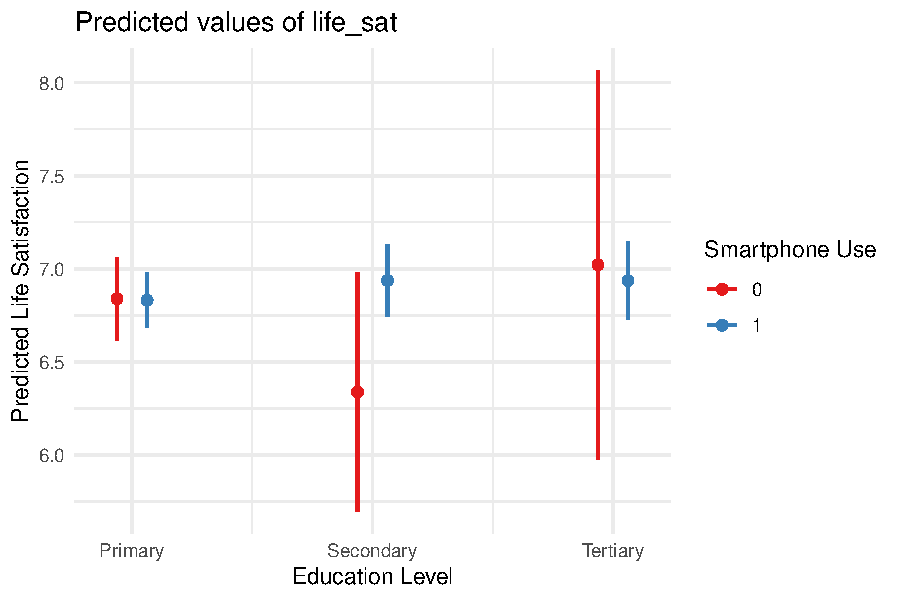
\includegraphics[keepaspectratio]{C:/Users/12545/Documents/WVS_report_final_files/output/smartphone_effects_files/figure-latex/predict-plot-1.pdf}}

\begin{Shaded}
\begin{Highlighting}[]
\NormalTok{df }\OtherTok{\textless{}{-}}\NormalTok{ df }\SpecialCharTok{\%\textgreater{}\%} \FunctionTok{mutate}\NormalTok{(}\AttributeTok{edu\_num =} \FunctionTok{as.numeric}\NormalTok{(education))}
\FunctionTok{ggplot}\NormalTok{(df, }\FunctionTok{aes}\NormalTok{(}\AttributeTok{x =}\NormalTok{ edu\_num, }\AttributeTok{y =}\NormalTok{ life\_sat,}
               \AttributeTok{color =} \FunctionTok{factor}\NormalTok{(phone\_use), }\AttributeTok{group =}\NormalTok{ phone\_use)) }\SpecialCharTok{+}
  \FunctionTok{geom\_jitter}\NormalTok{(}\AttributeTok{width =} \FloatTok{0.2}\NormalTok{, }\AttributeTok{alpha =} \FloatTok{0.3}\NormalTok{, }\AttributeTok{size =} \DecValTok{1}\NormalTok{) }\SpecialCharTok{+}
  \FunctionTok{geom\_smooth}\NormalTok{(}\AttributeTok{method =} \StringTok{"lm"}\NormalTok{, }\AttributeTok{se =} \ConstantTok{FALSE}\NormalTok{) }\SpecialCharTok{+}
  \FunctionTok{facet\_wrap}\NormalTok{(}\SpecialCharTok{\textasciitilde{}}\NormalTok{ female,}
             \AttributeTok{labeller =} \FunctionTok{labeller}\NormalTok{(}\AttributeTok{female =} \FunctionTok{c}\NormalTok{(}\StringTok{\textasciigrave{}}\AttributeTok{0}\StringTok{\textasciigrave{}}\OtherTok{=}\StringTok{"Male"}\NormalTok{, }\StringTok{\textasciigrave{}}\AttributeTok{1}\StringTok{\textasciigrave{}}\OtherTok{=}\StringTok{"Female"}\NormalTok{))) }\SpecialCharTok{+}
  \FunctionTok{scale\_x\_continuous}\NormalTok{(}\AttributeTok{breaks =} \DecValTok{1}\SpecialCharTok{:}\DecValTok{3}\NormalTok{,}
                     \AttributeTok{labels =} \FunctionTok{levels}\NormalTok{(df}\SpecialCharTok{$}\NormalTok{education)) }\SpecialCharTok{+}
  \FunctionTok{labs}\NormalTok{(}\AttributeTok{x =} \StringTok{"Education Level"}\NormalTok{,}
       \AttributeTok{y =} \StringTok{"Life Satisfaction"}\NormalTok{,}
       \AttributeTok{color =} \StringTok{"Smartphone Use"}\NormalTok{) }\SpecialCharTok{+}
  \FunctionTok{theme\_minimal}\NormalTok{()}
\end{Highlighting}
\end{Shaded}

\pandocbounded{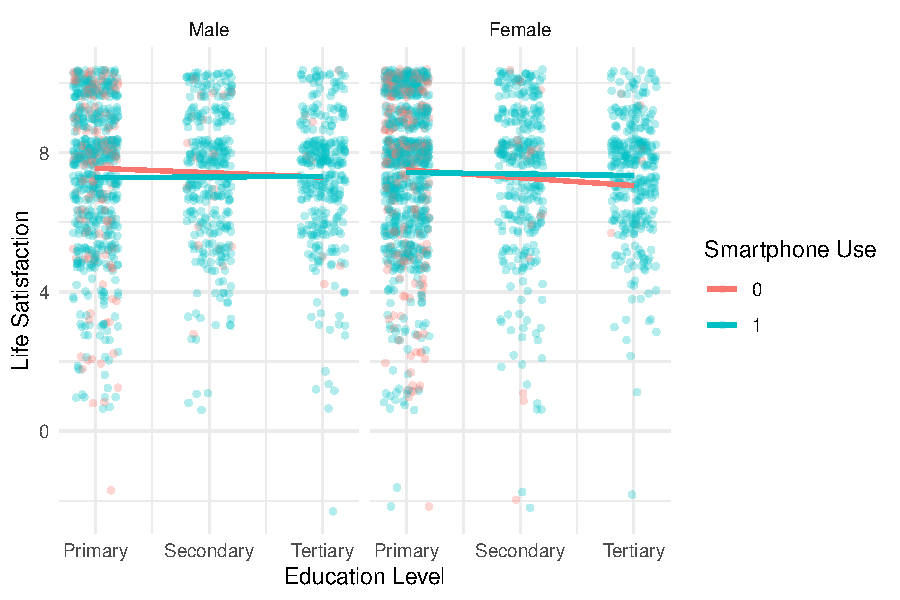
\includegraphics[keepaspectratio]{C:/Users/12545/Documents/WVS_report_final_files/output/smartphone_effects_files/figure-latex/facet-plot-enhanced-1.pdf}}

\begin{Shaded}
\begin{Highlighting}[]
\NormalTok{tbl }\OtherTok{\textless{}{-}} \FunctionTok{modelsummary}\NormalTok{(model, }\AttributeTok{output =} \StringTok{"data.frame"}\NormalTok{)}
\FunctionTok{kable}\NormalTok{(tbl, }\AttributeTok{caption =} \StringTok{"OLS Regression Results"}\NormalTok{, }\AttributeTok{booktabs =} \ConstantTok{TRUE}\NormalTok{) }\SpecialCharTok{\%\textgreater{}\%}
  \FunctionTok{kable\_styling}\NormalTok{(}\AttributeTok{full\_width =} \ConstantTok{FALSE}\NormalTok{, }\AttributeTok{position =} \StringTok{"left"}\NormalTok{) }\SpecialCharTok{\%\textgreater{}\%}
  \FunctionTok{row\_spec}\NormalTok{(}\DecValTok{0}\NormalTok{, }\AttributeTok{bold =} \ConstantTok{TRUE}\NormalTok{)}
\end{Highlighting}
\end{Shaded}

\begin{longtable}[l]{llll}
\caption{\label{tab:styled-table}OLS Regression Results}\\
\toprule
\textbf{part} & \textbf{term} & \textbf{statistic} & \textbf{(1)}\\
\midrule
estimates & (Intercept) & estimate & 5.685\\
estimates & (Intercept) & std.error & (0.218)\\
estimates & educationSecondary & estimate & -0.501\\
estimates & educationSecondary & std.error & (0.337)\\
estimates & educationTertiary & estimate & 0.183\\
\addlinespace
estimates & educationTertiary & std.error & (0.543)\\
estimates & phone\_use & estimate & -0.007\\
estimates & phone\_use & std.error & (0.121)\\
estimates & female & estimate & 0.099\\
estimates & female & std.error & (0.076)\\
\addlinespace
estimates & age & estimate & 0.025\\
estimates & age & std.error & (0.003)\\
estimates & income\_catMiddle & estimate & 0.776\\
estimates & income\_catMiddle & std.error & (0.081)\\
estimates & income\_catHigh & estimate & 1.391\\
\addlinespace
estimates & income\_catHigh & std.error & (0.239)\\
estimates & educationSecondary × phone\_use & estimate & 0.607\\
estimates & educationSecondary × phone\_use & std.error & (0.350)\\
estimates & educationTertiary × phone\_use & estimate & -0.077\\
estimates & educationTertiary × phone\_use & std.error & (0.549)\\
\addlinespace
gof & Num.Obs. &  & 2989\\
gof & R2 &  & 0.053\\
gof & R2 Adj. &  & 0.050\\
gof & AIC &  & 12790.3\\
gof & BIC &  & 12856.4\\
\addlinespace
gof & Log.Lik. &  & -6384.161\\
gof & RMSE &  & 2.05\\
\bottomrule
\end{longtable}

\begin{Shaded}
\begin{Highlighting}[]
\FunctionTok{sessionInfo}\NormalTok{()}
\end{Highlighting}
\end{Shaded}

\begin{verbatim}
## R version 4.5.0 (2025-04-11 ucrt)
## Platform: x86_64-w64-mingw32/x64
## Running under: Windows 11 x64 (build 26100)
## 
## Matrix products: default
##   LAPACK version 3.12.1
## 
## locale:
## [1] LC_COLLATE=Chinese (Simplified)_China.utf8 
## [2] LC_CTYPE=Chinese (Simplified)_China.utf8   
## [3] LC_MONETARY=Chinese (Simplified)_China.utf8
## [4] LC_NUMERIC=C                               
## [5] LC_TIME=Chinese (Simplified)_China.utf8    
## 
## time zone: Asia/Shanghai
## tzcode source: internal
## 
## attached base packages:
## [1] stats     graphics  grDevices utils     datasets  methods  
## [7] base     
## 
## other attached packages:
##  [1] rmarkdown_2.29     here_1.0.1         kableExtra_1.4.0  
##  [4] boot_1.3-31        estimatr_1.0.6     skimr_2.1.5       
##  [7] ggeffects_2.3.0    modelsummary_2.4.0 lubridate_1.9.4   
## [10] forcats_1.0.0      stringr_1.5.1      purrr_1.0.4       
## [13] readr_2.1.5        tidyr_1.3.1        tibble_3.2.1      
## [16] ggplot2_3.5.2      tidyverse_2.0.0    readxl_1.4.5      
## [19] semPlot_1.1.6      lavaan_0.6-19      dplyr_1.1.4       
## [22] haven_2.5.4       
## 
## loaded via a namespace (and not attached):
##   [1] rstudioapi_0.17.1   jsonlite_2.0.0      datawizard_1.1.0   
##   [4] magrittr_2.0.3      farver_2.1.2        nloptr_2.2.1       
##   [7] vctrs_0.6.5         minqa_1.2.8         base64enc_0.1-3    
##  [10] tinytex_0.57        htmltools_0.5.8.1   cellranger_1.1.0   
##  [13] Formula_1.2-5       htmlwidgets_1.6.4   plyr_1.8.9         
##  [16] igraph_2.1.4        lifecycle_1.0.4     pkgconfig_2.0.3    
##  [19] Matrix_1.7-3        R6_2.6.1            fastmap_1.2.0      
##  [22] rbibutils_2.3       digest_0.6.37       OpenMx_2.21.13     
##  [25] fdrtool_1.2.18      colorspace_2.1-1    rprojroot_2.0.4    
##  [28] textshaping_1.0.1   Hmisc_5.2-3         labeling_0.4.3     
##  [31] fansi_1.0.6         timechange_0.3.0    tinytable_0.9.0    
##  [34] abind_1.4-8         mgcv_1.9-1          compiler_4.5.0     
##  [37] withr_3.0.2         glasso_1.11         htmlTable_2.4.3    
##  [40] backports_1.5.0     carData_3.0-5       psych_2.5.3        
##  [43] performance_0.14.0  MASS_7.3-65         corpcor_1.6.10     
##  [46] gtools_3.9.5        tools_4.5.0         pbivnorm_0.6.0     
##  [49] foreign_0.8-90      zip_2.3.2           nnet_7.3-20        
##  [52] glue_1.8.0          quadprog_1.5-8      nlme_3.1-168       
##  [55] lisrelToR_0.3       grid_4.5.0          rsconnect_1.3.4    
##  [58] checkmate_2.3.2     cluster_2.1.8.1     reshape2_1.4.4     
##  [61] generics_0.1.3      gtable_0.3.6        tzdb_0.5.0         
##  [64] data.table_1.17.0   hms_1.1.3           xml2_1.3.8         
##  [67] sem_3.1-16          tables_0.9.31       pillar_1.10.2      
##  [70] rockchalk_1.8.157   splines_4.5.0       lattice_0.22-6     
##  [73] kutils_1.73         tidyselect_1.2.1    pbapply_1.7-2      
##  [76] knitr_1.50          reformulas_0.4.1    gridExtra_2.3      
##  [79] svglite_2.2.1       stats4_4.5.0        xfun_0.52          
##  [82] qgraph_1.9.8        arm_1.14-4          stringi_1.8.7      
##  [85] yaml_2.3.10         evaluate_1.0.3      mi_1.1             
##  [88] cli_3.6.4           RcppParallel_5.1.10 rpart_4.1.24       
##  [91] xtable_1.8-4        parameters_0.26.0   systemfonts_1.2.3  
##  [94] Rdpack_2.6.4        repr_1.1.7          munsell_0.5.1      
##  [97] Rcpp_1.0.14         coda_0.19-4.1       png_0.1-8          
## [100] XML_3.99-0.18       parallel_4.5.0      bayestestR_0.16.0  
## [103] jpeg_0.1-11         lme4_1.1-37         viridisLite_0.4.2  
## [106] scales_1.3.0        openxlsx_4.2.8      insight_1.3.0      
## [109] rlang_1.1.6         mnormt_2.1.1
\end{verbatim}

\subsection{Replication materials}\label{replication-materials}

All analysis code, the knitted PDF, and the one-line build script are
openly available on GitHub:\\
\url{https://github.com/Alex-Shen114514/WVS_report_final_files}

\begin{center}\rule{0.5\linewidth}{0.5pt}\end{center}

\end{document}
